\chapter{Perkembangbiakan Manusia}\label{ch:g5:human-reproduction}

Setiap orang yang kamu kenal --- teman, guru, orang tertua di
keluargamu --- tiba dengan cara yang sama: sebagai bayi, yang lahir
sesudah berbulan-bulan tumbuh di dalam tubuh ibunya. Manusia adalah
\omterm{prop:g3:sorting-living-things:groups}{mamalia} (\cref{prop:g4:classifying-animals:classes}), dan
perkembangbiakan manusia berjalan atas rancangan \omterm{prop:g3:sorting-living-things:groups}{mamalia} pada
\cref{ch:g4:animal-reproduction} --- dengan bilangan, tanggal dan
perincian \omterm{def:g5:biodiversity:species}{spesies} kita sendiri, yang dipaparkan bab ini dengan terus
terang.

\section{Versi manusia dari rancangannya}

\begin{proposition}[Perkembangbiakan manusia adalah perkembangbiakan mamalia]\label{prop:g5:human-reproduction:plan}
Seperti semua \omterm{prop:g3:sorting-living-things:groups}{mamalia}, manusia berkembang biak secara seksual
(\cref{def:g4:animal-reproduction:sexual}):
\begin{itemize}
  \item tubuh ibunya menghasilkan \emph{\omterm{def:g4:animal-reproduction:sexual}{sel telur}}; tubuh ayahnya
        menghasilkan \emph{\omterm{def:g4:animal-reproduction:sexual}{sel sperma}};
  \item \omterm{def:g5:flower-to-fruit:steps}{pembuahan} --- satu \omterm{def:g4:animal-reproduction:sexual}{sel sperma} yang bergabung dengan satu \omterm{def:g4:animal-reproduction:sexual}{sel
        telur} --- terjadi \emph{di dalam tubuh ibunya}
        (\cref{prop:g4:animal-reproduction:where});
  \item \omterm{def:g4:animal-reproduction:sexual}{sel telur} yang terbuahi --- satu \omterm{def:g5:first-look-at-cells:cell}{sel} tunggal
        (\cref{ex:g5:first-look-at-cells:one}) --- menetap di dalam
        \emph{rahim}\index{rahim} ibunya lalu tumbuh di situ;
  \item manusia bersifat \omterm{def:g4:animal-reproduction:ovivivi}{vivipar}
        (\cref{def:g4:animal-reproduction:ovivivi}): bayinya \omterm{def:g2:animals-grow-up:born}{lahir
        hidup}, dan mula-mula diberi makan dengan \omterm{def:g2:animals-grow-up:born}{susu}.
\end{itemize}
\end{proposition}
\admitted

\begin{remark}[Perkembangbiakan membutuhkan tubuh yang dewasa]\label{rem:g5:human-reproduction:adults}
Tubuh seorang anak tidak dapat membuat bayi: organ reproduksinya baru
mulai bekerja pada \emph{pubertas}, yaitu perubahan pada tahap \omterm{def:g3:stages-of-life:stages}{remaja}
\cref{def:g3:stages-of-life:stages}, ketika tubuhnya membangun ulang
dirinya dari tubuh anak menjadi tubuh orang dewasa. Apa yang diubah
pubertas, dan bagaimana caranya, adalah pokok satu bab penuh pada
tahun-tahun sekolah menengah pertama dalam buku ini.
\end{remark}

\section{Sembilan bulan di dalam rahim}

\begin{definition}[Kehamilan]\label{def:g5:human-reproduction:pregnancy}
Yang disebut \emph{kehamilan}\index{kehamilan} adalah waktu yang
dilewatkan calon bayi untuk tumbuh di dalam \omterm{prop:g5:human-reproduction:plan}{rahim} ibunya: kira-kira
\emph{sembilan bulan} pada manusia. Bayi yang sedang tumbuh itu
mula-mula disebut \emph{embrio}\index{embrio}, lalu --- begitu
rancangan tubuhnya terbentang, sesudah kira-kira dua bulan --- disebut
\emph{janin}\index{janin}.
\end{definition}

\begin{proposition}[Diberi makan lewat tali]\label{prop:g5:human-reproduction:cord}
Di dalam \omterm{prop:g5:human-reproduction:plan}{rahim}, bayinya mengapung di dalam sebuah kantong berisi
cairan dan tidak dapat makan atau bernapas. Segalanya datang siap
pakai dari \omterm{prop:g4:journey-of-food:absorb}{darah} ibunya: \omterm{def:g4:journey-of-food:digestion}{zat gizi} dan oksigen
(\cref{prop:g4:heart-and-blood:carries}) menyeberang ke dalam \omterm{prop:g4:journey-of-food:absorb}{darah}
bayinya lewat \emph{tali pusar}\index{tali pusar} di perutnya --- dan
buangannya menyeberang kembali lewat jalan yang sama, untuk ditangani
tubuh ibunya. Pusarmu adalah tempat tali pusarmu sendiri dahulu
melekat.
\end{proposition}
\admitted

\begin{example}[Jadwal sembilan bulan]\label{ex:g5:human-reproduction:timetable}
Bulan 1: segumpal \omterm{def:g5:first-look-at-cells:cell}{sel} yang membelah, lebih kecil daripada sebutir
beras, tetapi sudah tumbuh dengan cepat. Bulan 2: sebuah \omterm{def:g5:human-reproduction:pregnancy}{embrio} dengan
sketsa kepala, \omterm{def:g4:heart-and-blood:heart}{jantung} yang berdetak, tunas bagi \omterm{def:g1:my-body:parts}{lengan} dan \omterm{def:g1:my-body:parts}{tungkai}
--- masih lebih kecil daripada satu ibu jari. Bulan 3--4: sebuah
\omterm{def:g5:human-reproduction:pregnancy}{janin}, yang rancangannya sudah lengkap, mulai bergerak; ibunya segera
merasakan tendangannya. Bulan 5--8: tumbuh dan mematang ---
pendengarannya tiba, dan mantel rambut yang pertama. Bulan 9: bayinya,
yang biasanya berkepala di bawah dan berbobot sekitar \qty{3}{kg},
sudah siap.
\end{example}

\begin{example}[Kelahiran]\label{ex:g5:human-reproduction:birth}
Pada \omterm{def:g2:born-grow-die:cycle}{kelahiran}, \omterm{def:g3:bones-and-muscles:muscle}{otot} \omterm{prop:g5:human-reproduction:plan}{rahim} yang kuat mendorong bayinya keluar ke
dunia, biasanya dengan kepala lebih dahulu. Tangis pertamanya mengisi
\omterm{def:g4:breathing:organs}{paru-parunya} dengan udara --- \omterm{def:g4:breathing:organs}{paru-paru} itu belum pernah bernapas
sebelumnya (\cref{prop:g5:human-reproduction:cord}) --- \omterm{prop:g5:human-reproduction:cord}{tali pusarnya},
yang tidak lagi dibutuhkan, dipotong tanpa rasa sakit, dan rancangan
\omterm{prop:g3:sorting-living-things:groups}{mamalianya} berlanjut di luar: \omterm{def:g2:animals-grow-up:born}{susu}, kehangatan dan perawatan
(\cref{ex:g4:animal-reproduction:whalecalf} tentu menyetujuinya).
\end{example}

\begin{omfigure}
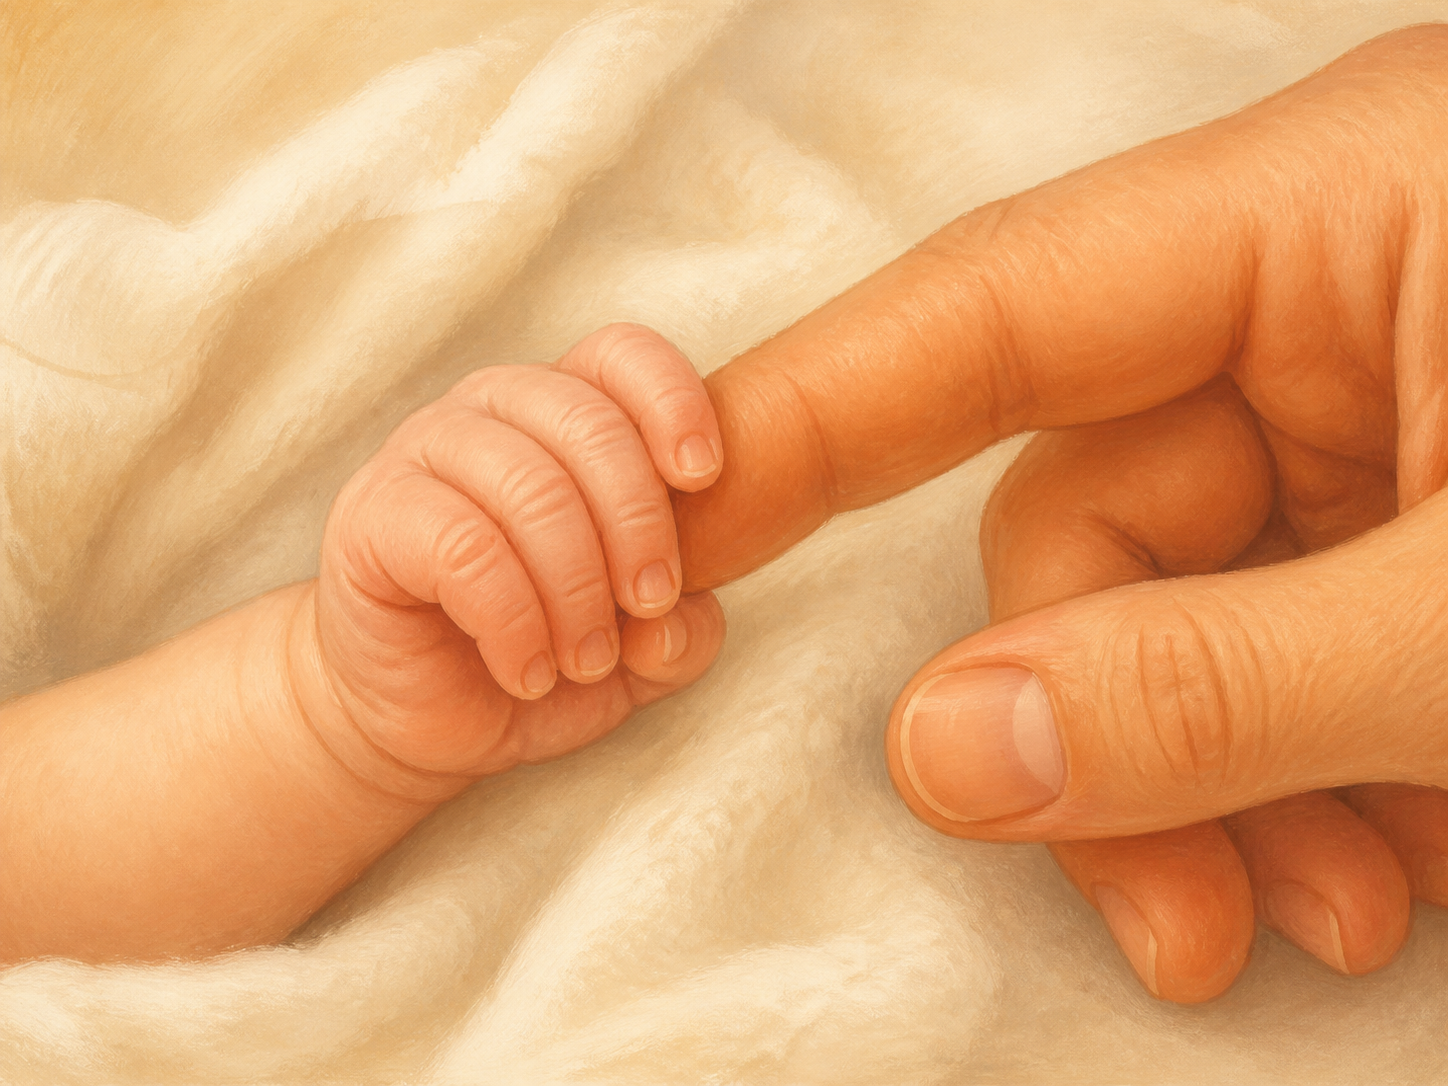
\includegraphics[width=0.52\linewidth]{images/book1/ai/g5-human-babyhand.png}

{\small Baru berumur beberapa hari, dan genggamannya sudah bekerja:
masa kanak-kanak manusia yang panjang bermula.}
\end{omfigure}

\begin{remark}[Anak kembar]\label{rem:g5:human-reproduction:twins}
Kadang dua bayi tumbuh bersama-sama di dalam \omterm{prop:g5:human-reproduction:plan}{rahim}. Kalau satu \omterm{def:g4:animal-reproduction:sexual}{sel
telur} yang terbuahi terbelah menjadi dua \omterm{def:g5:human-reproduction:pregnancy}{embrio}, kembarnya bersifat
\emph{identik} --- dibangun dari \omterm{def:g5:first-look-at-cells:cell}{sel} awal yang sama, serupa bagai dua
salinan. Kalau dua \omterm{def:g4:animal-reproduction:sexual}{sel telur} dibuahi oleh dua \omterm{def:g4:animal-reproduction:sexual}{sel sperma}, kembarnya
tidak lebih serupa daripada saudara kandung biasa --- keduanya hanya
berbagi \omterm{prop:g5:human-reproduction:plan}{rahim}. Dua jenis kembar, yang dibedakan oleh permulaannya.
\end{remark}

\section{Perawatan sebelum dan sesudahnya}

\begin{proposition}[Bayinya berbagi persediaan ibunya]\label{prop:g5:human-reproduction:care}
Segala yang mencapai bayinya mengembara lewat \omterm{prop:g4:journey-of-food:absorb}{darah} ibunya --- itulah
sebabnya seorang ibu yang sedang mengandung makan dengan baik
(\cref{ch:g3:balanced-diet}), beristirahat, diikuti oleh dokter atau
bidan, dan menghindari apa yang dapat membahayakan bayinya: asap
tembakau dan alkohol pun melintas lewat \omterm{prop:g5:human-reproduction:cord}{tali pusarnya}, dan seorang
\omterm{def:g5:human-reproduction:pregnancy}{janin} jauh lebih rapuh daripada orang dewasa. Merawat ibunya
\emph{berarti} merawat bayinya.
\end{proposition}
\admitted

\begin{example}[Sebuah spesies yang sangat terawat]\label{ex:g5:human-reproduction:longcare}
Bahkan di antara \omterm{prop:g3:sorting-living-things:groups}{mamalia}, manusia mendorong siasat sedikit-dan-terawat
pada \cref{prop:g4:animal-reproduction:strategies} sampai ujungnya:
biasanya satu bayi dalam satu waktu, tak berdaya jauh lebih lama
daripada anak kuda atau anak kucing, dan dirawat --- diberi makan,
diajar, disayangi --- selama \emph{bertahun-tahun}. Masa kanak-kanak manusia
adalah salah satu yang terpanjang di dunia \omterm{def:g1:animals-around-us:animal}{hewan}; buku ini, sebuah
kursus sepanjang sepuluh tahun, sendiri merupakan sekeping dari
perawatan yang panjang itu.
\end{example}

\section{Latihan}

\begin{exercise}[$\star$]\label{exo:g5:human-reproduction:1}
\omterm{def:g5:first-look-at-cells:cell}{Sel} mana yang datang dari ibunya, mana dari ayahnya, dan penggabungan
keduanya disebut apa?
\end{exercise}

\begin{exercise}[$\star$]\label{exo:g5:human-reproduction:2}
Di mana bayi manusia tumbuh, dan kira-kira selama berapa lama?
\end{exercise}

\begin{exercise}[$\star$]\label{exo:g5:human-reproduction:3}
Apa kedua nama bayi yang sedang tumbuh itu, berurutan, dan kira-kira
kapan yang pertama menjadi yang kedua?
\end{exercise}

\begin{exercise}[$\star$]\label{exo:g5:human-reproduction:4}
Bayi di dalam \omterm{prop:g5:human-reproduction:plan}{rahim} tidak makan dan tidak bernapas. Bagaimana ia
memperoleh \omterm{def:g4:journey-of-food:digestion}{zat gizi} dan oksigen, dan ke mana buangannya pergi?
\end{exercise}

\begin{exercise}[$\star$]\label{exo:g5:human-reproduction:5}
Pusarmu adalah tanda dari apa?
\end{exercise}

\begin{exercise}[$\star$]\label{exo:g5:human-reproduction:6}
Apa yang terjadi pada tangis pertama, dan mengapa itu perubahan yang
begitu besar bagi tubuh bayinya?
\end{exercise}

\begin{exercise}[$\star$]\label{exo:g5:human-reproduction:7}
Ciri mana saja yang membuat perkembangbiakan manusia khas \omterm{prop:g3:sorting-living-things:groups}{mamalia}?
Sebutkan tiga, dengan mengutip
\cref{prop:g4:classifying-animals:classes} atau
\cref{ch:g4:animal-reproduction}.
\end{exercise}

\begin{exercise}[$\star$]\label{exo:g5:human-reproduction:8}
Mengapa dokter meminta ibu yang sedang mengandung menghindari asap
tembakau dan alkohol? Pakai \cref{prop:g5:human-reproduction:care}.
\end{exercise}

\begin{exercise}[$\star\star$]\label{exo:g5:human-reproduction:9}
Jelaskan kedua jenis kembar menurut permulaannya. Jenis mana yang
serupa ``bagai dua salinan'', dan mengapa hal itu mengikuti dari
\cref{ex:g5:first-look-at-cells:one}?
\end{exercise}

\begin{exercise}[$\star\star$]\label{exo:g5:human-reproduction:10}
Tempatkan manusia pada garis siasat
\cref{prop:g4:animal-reproduction:strategies}, dengan membandingkannya
dengan \omterm{prop:g3:sorting-living-things:groups}{ikan} kod dan gajah: jumlah anak, lamanya perawatan, dan apa isi
perawatan yang panjang itu bagi manusia.
\end{exercise}

\begin{exercise}[$\star\star\star$]\label{exo:g5:human-reproduction:11}
Pada \omterm{def:g2:born-grow-die:cycle}{kelahiran}, \omterm{prop:g5:human-reproduction:cord}{tali pusar} yang dipotong mengakhiri jalur pasokan
bayinya tepat pada saat \omterm{def:g4:breathing:organs}{paru-parunya} \omterm{def:g4:breathing:movements}{menarik napas} pertamanya. Dengan
memakai \cref{prop:g5:human-reproduction:cord} dan
\cref{prop:g4:breathing:exchange}, jelaskan tugas apa yang beralih,
pada menit itu, dari tubuh ibunya ke \omterm{def:g4:breathing:organs}{paru-paru} bayinya sendiri --- dan
mengapa tangis pertamanya tepat waktu.
\end{exercise}
